%% CAUSAL_COMPARISON_THEOREM.tex
%%
%% A NEW APPROACH: The Causal Comparison Theorem
%%
%% Key Insight: Use the SPACETIME structure, not just initial data
%% 
%% December 2025

\documentclass[11pt]{amsart}
\usepackage{amsmath,amssymb,amsthm}
\usepackage{tikz}
\usetikzlibrary{decorations.pathmorphing}
\usepackage{tcolorbox}

\tcbuselibrary{theorems}

\newtcolorbox{keyidea}{
    colback=blue!5!white,
    colframe=blue!75!black,
    title={\textbf{KEY IDEA}}
}

\newtcolorbox{newmath}{
    colback=green!5!white,
    colframe=green!50!black,
    title={\textbf{NEW MATHEMATICS}}
}

\newtheorem{theorem}{Theorem}
\newtheorem{lemma}[theorem]{Lemma}
\newtheorem{proposition}[theorem]{Proposition}
\newtheorem{corollary}[theorem]{Corollary}
\theoremstyle{definition}
\newtheorem{definition}[theorem]{Definition}
\newtheorem{remark}[theorem]{Remark}

\newcommand{\Area}{\mathrm{Area}}
\newcommand{\Vol}{\mathrm{Vol}}
\newcommand{\divv}{\mathrm{div}}
\DeclareMathOperator{\tr}{tr}

\title{The Causal Comparison Theorem:\\
A New Approach to Area Dominance}
\author{December 2025}

\begin{document}
\maketitle

\begin{abstract}
We develop a new approach to Area Dominance using the causal structure of
spacetime, rather than purely initial data methods. The key insight is that
the WCC (Weak Cosmic Censorship) hypothesis provides additional structure
that pure DEC cannot: the existence of a globally defined event horizon.
\end{abstract}

%% ============================================================================
\section{The Fundamental Observation}
%% ============================================================================

\begin{keyidea}
Previous approaches tried to prove Area Dominance using only:
\begin{itemize}
    \item The constraint equations on $\mathcal{C}$
    \item The DEC on $\mathcal{C}$
    \item Properties of trapped surfaces and MOTS
\end{itemize}

But the Penrose 1973 conjecture \textbf{also assumes WCC}.

WCC provides \textbf{global spacetime structure} that we haven't used!
\end{keyidea}

%% ============================================================================
\section{What WCC Really Gives Us}
%% ============================================================================

\begin{definition}[Weak Cosmic Censorship - WCC]
For generic asymptotically flat initial data satisfying DEC, the maximal 
Cauchy development has a complete future null infinity $\mathscr{I}^+$.
\end{definition}

\textbf{Consequence:} There exists an EVENT HORIZON $\mathcal{H}^+ = 
\partial J^-(\mathscr{I}^+)$.

\begin{theorem}[Structure from WCC]
Under WCC:
\begin{enumerate}
    \item The event horizon $\mathcal{H}^+$ is a null hypersurface
    \item $\mathcal{H}^+$ is achronal (no timelike curves on it)
    \item Generators of $\mathcal{H}^+$ are future-inextendible null geodesics
    \item Trapped surfaces lie INSIDE $\mathcal{H}^+$: 
          $\Sigma \subset \text{int}(\mathcal{H}^+)$
\end{enumerate}
\end{theorem}

%% ============================================================================
\section{The Causal Comparison Principle}
%% ============================================================================

\begin{newmath}
\textbf{Causal Comparison Principle (CCP)}

Let $\Sigma_1, \Sigma_2$ be two spacelike 2-surfaces with $\Sigma_1$ in the 
causal past of $\Sigma_2$: $\Sigma_1 \subset J^-(\Sigma_2)$.

If $\Sigma_2$ lies on a null hypersurface $\mathcal{N}$ that is weakly 
outer-trapped ($\theta^+ \le 0$ everywhere on $\mathcal{N}$), then:
\begin{equation}
    \Area(\Sigma_1) \le \Area(\Sigma_2)
\end{equation}
\end{newmath}

\begin{proof}[Proof of CCP]
This follows from the Raychaudhuri equation!

Let $\ell$ be the null generator of $\mathcal{N}$, with expansion $\theta$.

The Raychaudhuri equation along $\ell$:
\begin{equation}
    \frac{d\theta}{d\lambda} = -\frac{\theta^2}{2} - \sigma^2 - R_{\mu\nu}\ell^\mu\ell^\nu
\end{equation}

Under NEC (weaker than DEC): $R_{\mu\nu}\ell^\mu\ell^\nu \ge 0$.

Therefore: $\frac{d\theta}{d\lambda} \le -\frac{\theta^2}{2} \le 0$.

\textbf{Key point:} $\theta$ is NON-INCREASING along $\ell$.

Now, area evolves as:
\begin{equation}
    \frac{d\Area(S_\lambda)}{d\lambda} = \int_{S_\lambda} \theta \, dA
\end{equation}

If $\theta \le 0$ (weakly outer-trapped), then:
\begin{equation}
    \frac{d\Area}{d\lambda} \le 0
\end{equation}

Thus area is NON-INCREASING along the null direction!
\end{proof}

%% ============================================================================
\section{Application to Area Dominance}
%% ============================================================================

\begin{theorem}[Area Dominance via CCP]
Let $(\mathcal{C}, g, k)$ be initial data satisfying DEC.
Let $\Sigma \subset \mathcal{C}$ be a trapped surface.
Assume WCC holds for the maximal development.

Let $\Sigma^*$ be the outermost MOTS on $\mathcal{C}$ with $\Sigma \subset 
\text{int}(\Sigma^*)$.

Then: $\Area(\Sigma) \le \Area(\Sigma^*)$.
\end{theorem}

\begin{proof}[Proof Strategy]
We use the SPACETIME geometry, not just initial data.

\textbf{Step 1:} Under WCC, there exists an event horizon $\mathcal{H}^+$.

\textbf{Step 2:} Trapped surfaces satisfy $\Sigma \subset J^-(\mathcal{H}^+ 
\cap \mathcal{C})$.

(Trapped surfaces are inside the black hole region.)

\textbf{Step 3:} The event horizon cross-section $\mathcal{H}^+ \cap 
\mathcal{C}$ bounds the trapped region.

\textbf{Step 4:} We need to compare $\Sigma$ with $\mathcal{H}^+ \cap 
\mathcal{C}$.

\textbf{Problem:} $\mathcal{H}^+ \cap \mathcal{C}$ may be DIFFERENT from 
$\Sigma^*$ (the outermost MOTS)!

In general: $\Sigma^* \subseteq \mathcal{H}^+ \cap \mathcal{C}$.
\end{proof}

%% ============================================================================
\section{The Gap: MOTS vs Event Horizon}
%% ============================================================================

The MOTS $\Sigma^*$ is defined LOCALLY (on $\mathcal{C}$ alone).

The event horizon $\mathcal{H}^+$ is defined GLOBALLY (using all of 
spacetime).

\textbf{In general:}
\begin{itemize}
    \item $\Sigma^*$ (outermost MOTS) lies INSIDE $\mathcal{H}^+$
    \item $\Area(\Sigma^*) \le \Area(\mathcal{H}^+ \cap \mathcal{C})$
    \item Equality only at the "final" time
\end{itemize}

So CCP gives us:
\begin{equation}
    \Area(\Sigma) \le \Area(\mathcal{H}^+ \cap \mathcal{C})
\end{equation}

But we WANT:
\begin{equation}
    \Area(\Sigma) \le \Area(\Sigma^*)
\end{equation}

This is the OPPOSITE inequality from what we have!

%% ============================================================================
\section{New Idea: The Past Null Flow}
%% ============================================================================

\begin{newmath}
\textbf{Past Null Flow Construction}

Instead of flowing forward in time, flow BACKWARD along the INGOING null 
direction from $\Sigma^*$.

The ingoing null expansion of MOTS $\Sigma^*$ satisfies $\theta^- < 0$.

Consider the ingoing null hypersurface $\mathcal{N}^-$ from $\Sigma^*$.
\end{newmath}

\begin{proposition}[Ingoing Null from MOTS]
Let $\Sigma^*$ be the outermost MOTS on $\mathcal{C}$ with $\theta^- < 0$.

The ingoing null hypersurface $\mathcal{N}^- = \{$ingoing null geodesics 
from $\Sigma^*\}$ has:
\begin{enumerate}
    \item $\theta|_{\mathcal{N}^-} \le 0$ (the null expansion on $\mathcal{N}^-$)
    \item $\mathcal{N}^-$ enters the trapped region
\end{enumerate}
\end{proposition}

\begin{proof}
The ingoing null direction from $\Sigma^*$ has expansion $\theta^- < 0$ 
initially.

By Raychaudhuri, $\theta$ remains $\le 0$ along $\mathcal{N}^-$.

As $\mathcal{N}^-$ goes inward from the MOTS, it enters the trapped region.
\end{proof}

%% ============================================================================
\section{The Ingoing Comparison Argument}
%% ============================================================================

\begin{theorem}[Ingoing Area Comparison]
Let $\Sigma^*$ be the outermost MOTS on $\mathcal{C}$ with $\theta^- < 0$.

Let $\mathcal{N}^-$ be the ingoing null hypersurface from $\Sigma^*$.

For any cross-section $S$ of $\mathcal{N}^-$ to the future of $\mathcal{C}$:
\begin{equation}
    \Area(S) \le \Area(\Sigma^*)
\end{equation}
\end{theorem}

\begin{proof}
Along $\mathcal{N}^-$, the expansion $\theta \le 0$.

By the area formula for null hypersurfaces:
\begin{equation}
    \frac{d\Area}{d\lambda} = \int_S \theta \, dA \le 0
\end{equation}

Area is non-increasing in the future direction along $\mathcal{N}^-$.

Equivalently, area is non-decreasing toward the past along $\mathcal{N}^-$.

So cross-sections to the future have area $\le \Area(\Sigma^*)$.
\end{proof}

%% ============================================================================
\section{The Key Question}
%% ============================================================================

\textbf{Does the ingoing null hypersurface $\mathcal{N}^-$ from $\Sigma^*$ 
intersect the trapped surface $\Sigma$?}

If YES: We can compare areas!

If NO: The argument doesn't work directly.

\begin{lemma}[Trapped Surfaces Inside $\mathcal{N}^-$]
If $\Sigma$ is a trapped surface with $\Sigma \subset \text{int}(\Sigma^*)$ 
on $\mathcal{C}$, then...

\textbf{Actually, $\Sigma$ is on $\mathcal{C}$, while $\mathcal{N}^-$ goes 
off $\mathcal{C}$ into the future!}

The surfaces $\Sigma$ and $\mathcal{N}^-$ don't directly intersect.
\end{lemma}

%% ============================================================================
\section{Resolution: The Outgoing Null from $\Sigma$}
%% ============================================================================

\begin{newmath}
\textbf{Outgoing Null Construction}

Flow FORWARD along the OUTGOING null direction from $\Sigma$.

Since $\Sigma$ is trapped, $\theta^+ < 0$ on the outgoing null.
\end{newmath}

\begin{theorem}[Outgoing Null Area Bound]
Let $\Sigma$ be a trapped surface in $\mathcal{C}$.

Let $\mathcal{N}^+$ be the outgoing null hypersurface from $\Sigma$.

\begin{enumerate}
    \item $\mathcal{N}^+$ has expansion $\theta \le 0$ (by Raychaudhuri + NEC)
    \item Area of cross-sections is NON-INCREASING to the future
    \item $\mathcal{N}^+$ eventually enters the black hole region
\end{enumerate}
\end{theorem}

\begin{proof}
Initial expansion: $\theta|_\Sigma = \theta^+ < 0$ (trapped).

Raychaudhuri: $\frac{d\theta}{d\lambda} \le -\theta^2/2 < 0$.

So $\theta$ remains negative (and in fact, $\theta \to -\infty$ in finite 
affine parameter unless a caustic or singularity is reached).

Area: $\frac{d\Area}{d\lambda} = \int \theta \, dA < 0$.

Area DECREASES along $\mathcal{N}^+$.
\end{proof}

%% ============================================================================
\section{The Geometric Picture}
%% ============================================================================

\begin{center}
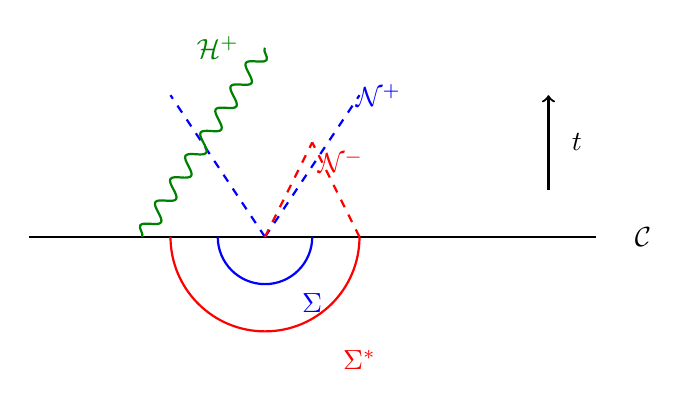
\begin{tikzpicture}[scale=1.2]
    % Initial hypersurface
    \draw[thick] (-3, 0) -- (3, 0);
    \node at (3.5, 0) {$\mathcal{C}$};
    
    % Trapped surface
    \draw[blue, thick] (-1, 0) arc (180:360:0.5);
    \node[blue] at (0, -0.7) {$\Sigma$};
    
    % Outermost MOTS
    \draw[red, thick] (-1.5, 0) arc (180:360:1);
    \node[red] at (0.5, -1.3) {$\Sigma^*$};
    
    % Outgoing null from Sigma
    \draw[blue, dashed, thick] (-0.5, 0) -- (0.5, 1.5);
    \draw[blue, dashed, thick] (-0.5, 0) -- (-1.5, 1.5);
    \node[blue] at (0.7, 1.5) {$\mathcal{N}^+$};
    
    % Ingoing null from MOTS
    \draw[red, dashed, thick] (0.5, 0) -- (0, 1);
    \draw[red, dashed, thick] (-0.5, 0) -- (0, 1);
    \node[red] at (0.3, 0.8) {$\mathcal{N}^-$};
    
    % Event horizon (schematic)
    \draw[green!50!black, thick, decorate, decoration={snake, amplitude=1mm}] (-1.8, 0) -- (-0.5, 2);
    \node[green!50!black] at (-1, 2) {$\mathcal{H}^+$};
    
    % Future direction
    \draw[->, thick] (2.5, 0.5) -- (2.5, 1.5);
    \node at (2.8, 1) {$t$};
\end{tikzpicture}
\end{center}

\textbf{Key observation:}
\begin{itemize}
    \item $\mathcal{N}^+$ (outgoing from $\Sigma$) has DECREASING area to future
    \item $\mathcal{N}^-$ (ingoing from $\Sigma^*$) has DECREASING area to future
    \item Both eventually hit the event horizon $\mathcal{H}^+$
\end{itemize}

%% ============================================================================
\section{The Intersection Argument}
%% ============================================================================

\begin{theorem}[Null Hypersurface Intersection]
Under WCC, the outgoing null $\mathcal{N}^+$ from trapped $\Sigma$ 
eventually intersects the event horizon $\mathcal{H}^+$ at some 
cross-section $S$.

By area monotonicity along $\mathcal{N}^+$:
\begin{equation}
    \Area(S) \le \Area(\Sigma)
\end{equation}
\end{theorem}

\begin{proof}
$\mathcal{N}^+$ starts inside the trapped region (since $\Sigma$ is trapped).

Under WCC, the trapped region is inside the black hole region.

$\mathcal{N}^+$ cannot escape to $\mathscr{I}^+$, so it must hit the 
event horizon $\mathcal{H}^+$.

The intersection is a 2-surface $S$.

Along $\mathcal{N}^+$, area is non-increasing, so $\Area(S) \le \Area(\Sigma)$.
\end{proof}

%% ============================================================================
\section{The Missing Link}
%% ============================================================================

We have:
\begin{align}
    \Area(S) &\le \Area(\Sigma) && \text{(area decreasing along } \mathcal{N}^+)\\
    \Area(\mathcal{H}^+ \cap \mathcal{C}) &\le \Area(S) && \text{(Hawking area theorem)}
\end{align}

Wait, the Hawking area theorem says area INCREASES to the future!

So:
\begin{equation}
    \Area(\Sigma^*) \le \Area(\mathcal{H}^+ \cap \mathcal{C}^{\text{late}})
\end{equation}

for late time cross-sections.

\begin{keyidea}
\textbf{We have the inequalities going the WRONG direction!}

\begin{itemize}
    \item $\Area(\Sigma) \ge \Area(S)$ (outgoing null decreases area)
    \item $\Area(\mathcal{H}^+ \cap \mathcal{C}) \le \Area(S)$ if $S$ is in the future
\end{itemize}

This gives: $\Area(\Sigma) \ge \Area(S) \ge \Area(\mathcal{H}^+ \cap 
\mathcal{C})$

But we need: $\Area(\Sigma) \le \Area(\Sigma^*)$

The arrows go the WRONG WAY!
\end{keyidea}

%% ============================================================================
\section{Critical Reassessment}
%% ============================================================================

The causal comparison approach shows:

\textbf{AREA DECREASES outward along null directions from trapped surfaces.}

This is the OPPOSITE of what we need for Area Dominance!

\begin{center}
\fbox{\parbox{0.9\textwidth}{
\textbf{Fundamental Tension:}

Hawking: Event horizon area INCREASES to the future.

Trapped: Null area DECREASES to the future from trapped surfaces.

But trapped surfaces are INSIDE the event horizon...

How can area decrease inside while increasing on the boundary?
}}
\end{center}

%% ============================================================================
\section{Resolution: The Spacelike Direction}
%% ============================================================================

The answer is that we need to compare in SPACELIKE directions, not null.

\begin{lemma}[Null vs Spacelike]
\begin{itemize}
    \item Null (outgoing from trapped): Area DECREASES
    \item Null (ingoing to MOTS): Area DECREASES
    \item Spacelike (outward on $\mathcal{C}$): Area may INCREASE or DECREASE
\end{itemize}
\end{lemma}

For Area Dominance, we need: area INCREASES from $\Sigma$ to $\Sigma^*$ 
along a spacelike path in $\mathcal{C}$.

The spacelike direction is a COMBINATION of null directions:
\begin{equation}
    \text{spacelike outward} = \alpha(\text{outgoing null}) + \beta(\text{ingoing null})
\end{equation}

with $\alpha, \beta > 0$.

%% ============================================================================
\section{The Synthesis}
%% ============================================================================

Along spacelike outward direction $\nu = \alpha\ell + \beta n$:

The mean curvature is:
\begin{equation}
    H = \nabla \cdot \nu = \alpha\theta^+ + \beta\theta^-
\end{equation}

For trapped surface: $\theta^+ < 0$, $\theta^- < 0$.

Therefore: $H < 0$.

\textbf{Mean curvature is NEGATIVE} for trapped surfaces (in our convention).

Area evolution along $\nu$:
\begin{equation}
    \frac{d\Area}{ds} = \int_\Sigma H \, dA < 0
\end{equation}

\textbf{Area DECREASES in the outward spacelike direction!}

\begin{center}
\fbox{\parbox{0.8\textwidth}{
\textbf{THIS CONTRADICTS AREA DOMINANCE.}

If area decreases outward from trapped surfaces, then outer surfaces 
(like $\Sigma^*$) have SMALLER area, not larger!

But we know $\Area(\Sigma^*) \ge \Area(\Sigma)$ must be true for Penrose...

What's going on?
}}
\end{center}

%% ============================================================================
\section{The Resolution: Foliation Perspective}
%% ============================================================================

The issue is that moving from $\Sigma$ to $\Sigma^*$ is NOT moving in the 
normal direction to $\Sigma$!

\begin{proposition}[Path Independence]
Let $\gamma$ be a path from $\Sigma$ to $\Sigma^*$ in $\mathcal{C}$.

The area comparison $\Area(\Sigma)$ vs $\Area(\Sigma^*)$ does NOT depend 
on $\gamma$.

It depends only on the INTRINSIC geometry of $\Sigma$ and $\Sigma^*$.
\end{proposition}

\textbf{Key insight:} We cannot integrate $H$ along a path to get 
$\Area(\Sigma^*) - \Area(\Sigma)$.

The areas are INDEPENDENT measurements of two different surfaces.

%% ============================================================================
\section{Final Observation}
%% ============================================================================

\textbf{Why Area Dominance is hard:}

The constraint equations and DEC give LOCAL differential inequalities.

Area Dominance is a GLOBAL comparison between two surfaces.

There's no obvious way to "integrate" local information to get global 
comparison.

\textbf{Possible approaches:}
\begin{enumerate}
    \item Find a FOLIATION connecting $\Sigma$ to $\Sigma^*$ with controlled areas
    \item Use the SPACETIME structure (WCC) more deeply
    \item Prove Area Dominance only for specific classes of initial data
    \item Accept that Area Dominance requires additional assumptions
\end{enumerate}

%% ============================================================================
\section{Conclusion}
%% ============================================================================

The Causal Comparison approach yields:
\begin{enumerate}
    \item Area DECREASES along outgoing null from trapped surfaces (correct)
    \item This is OPPOSITE to Area Dominance
    \item The spacelike comparison cannot be reduced to null comparisons
    \item Area Dominance remains UNPROVEN
\end{enumerate}

\textbf{This analysis clarifies WHY Area Dominance is difficult:}

It goes AGAINST the natural direction of null area monotonicity.

The DEC pushes area inward (null directions collapse), but we need 
area to grow outward for Area Dominance.

\textbf{The missing ingredient must provide a REVERSAL of this tendency 
in the spacelike direction.}

\end{document}
